This chapter presents the results of our research into the technical
underpinnings of the Kinect as a sensing device. Section~\ref{howitworks}
describes techniques implemented in the Kinect to produce depth maps, in terms
of standard concepts from the field of machine vision. %Then, section
%\ref{precision} presents measurements, estimates and published data, which
%together characterise the precision of the Kinect as a measurement tool.

\section{Overview: What is a Kinect}

The Kinect device is a sensor array incorporating, most notably, a system for
depth measurement. This system relies on a technique that enables low-cost
implementations. Several founders of an Israeli technology firm, PrimeSense Ltd,
invented the technique sometime before 11 October 2005 \cite{ZALEVSKY:2007}.
Microsoft corp., in turn, began selling the Kinect-branded implementation on 10
November 2010 as an optional user interface for its consumer gaming platform,
the Xbox 360.


\subsection{Specifications}

Table~\ref{tab:specs} on page~\pageref{tab:specs} provides an overview of the
electronic components that comprise the Kinect's sensor array.

\begin{table}[ht]
\centering
\begin{tabular}{l p{10cm}}
\toprule
Component & Description \\
\midrule

RGB Camera & Sensor ``very similar'' to Mi\-cron mt9v112 (1/6" VGA CMOS) but
``larger'' and with some di\-ffering reg\-isters. Bay\-er co\-lour pa\-ttern (RG,GB).
640x\-480 pixels, 8-bit at 30 Hz.  1280x\-1024 pixels at 10\-Hz if using Open\-NI backend
, though this is referred to as ``15Hz'' in low level pro\-tocol. UYVY co\-lour
for\-mat also possible at ``15 Hz'' framerate.\cite{FREENECT}\cite{RGBDEMO} \\

Infrared camera & Monochrome CMOS sensor (no reliable source for this). Three
options for pixel size: ``small'' (unspecified); 640x480; 1280x1024. Framerate
options are 15Hz and 30Hz, except at maximum resolution (~9Hz).\cite{FREENECT}
field of view at 57 degrees horizontal, 43 degrees vertical according to retail
description.\cite{PLAY} Range reportedly ``adjustable'' (unconfirmed source) \\ 

Depth stream & Uncompressed data stream 16 bits, though this causes device
bandwidth problems. Usable options: ``differential/RLE'' compressed 11-bit
stream; 10-bit stream; 11-bit stream (uncompressed? still to be confirmed). The
only usable pixel size is 640x480. Framerate: 30Hz. \cite{FREENECT} Depth range
1.2m to 3.5m according to retail description.\cite{PLAY} Actual range
capability: ~ 0.7m-0.6m (unconfirmed source).\\

Infrared projector & Although non-reliable internet sources refer to the use of
a ``laser'' to project the infrared speckle pattern, this is unconfirmed. One
patent application relating to the Kinect describes a projecting a ``pattern of
coherent radiation''.\cite{SHPUNT:2010-1} Section \ref{howitworks} provides more
detail regading the projection component. \\

Accelerometer & Kionix KXSD9 Series. Sensitivity: 819 counts per g of
acceleration. Reports device tilt relative to the
horizon.\cite{FREENECT}\cite{KIONIX}\\

Microphone & ``Multiarray'' microphone consisting of four microphone units. Each
microphone generates two streams of 32 bit signed little endian PCM samples at
16KHz. A ninth channel from the device provides a unified noise-cancelled signal
in 16-bit little endian PCM samples (16KHz).\cite{FREENECT}\\

\bottomrule
\end{tabular}
\caption{Specifications of the Kinect}
\label{tab:specs}
\end{table}


\section{Theory: How it works}
\label{howitworks}

This sections describes the depth measurement implementation in relatively
high level terms, from the perspective of theoretical computer vision. These
descriptions are based on our interpretation of public records, including
patents and scholarly as well as casual articles. We also refer, though to a
lesser extent, to our own experiments with the Kinect.


\subsection{Overview: building depth images}

Our assessment is that, irrespective of the precise techniques employed, the
Kinect uses the following general recipe, implemented in some form of a
pipeline, to produce depth images: First, the projector projects speckle
patterns into a scene. Second, the infrared camera produces images that show the
speckle pattern (c.f.\ figure~\ref{fig:pattern1} on
page~\pageref{fig:pattern1}), as it reflects from the surfaces of objects in the
scene. By using a bandpass filter targeted at the wavelength of the projected
light, the image shows the speckle pattern with high contrast and relatively
little noise. Third: for each subregion of the image, the device employs one or
more approaches to solving the so-called ``correspondence problem'' (c.f.\
section~\ref{sub:corr} below), to find the matching subregion in a reference
image stored in memory. The resulting disparity value, $d_i$, is written into a
disparity image. The device then iterates over the disparity image and employs
triangulation (c.f.\ sections \ref{sub:triang} and \ref{sub:atriang} below) to
derive the depth value for each subregion, $Z_a$, which it writes to a depth
image. The following sections first describe the triangulation method, before
going on to discuss potential solutions to the ``correspondence problem''.

\begin{figure}[ht]
    \begin{center}
        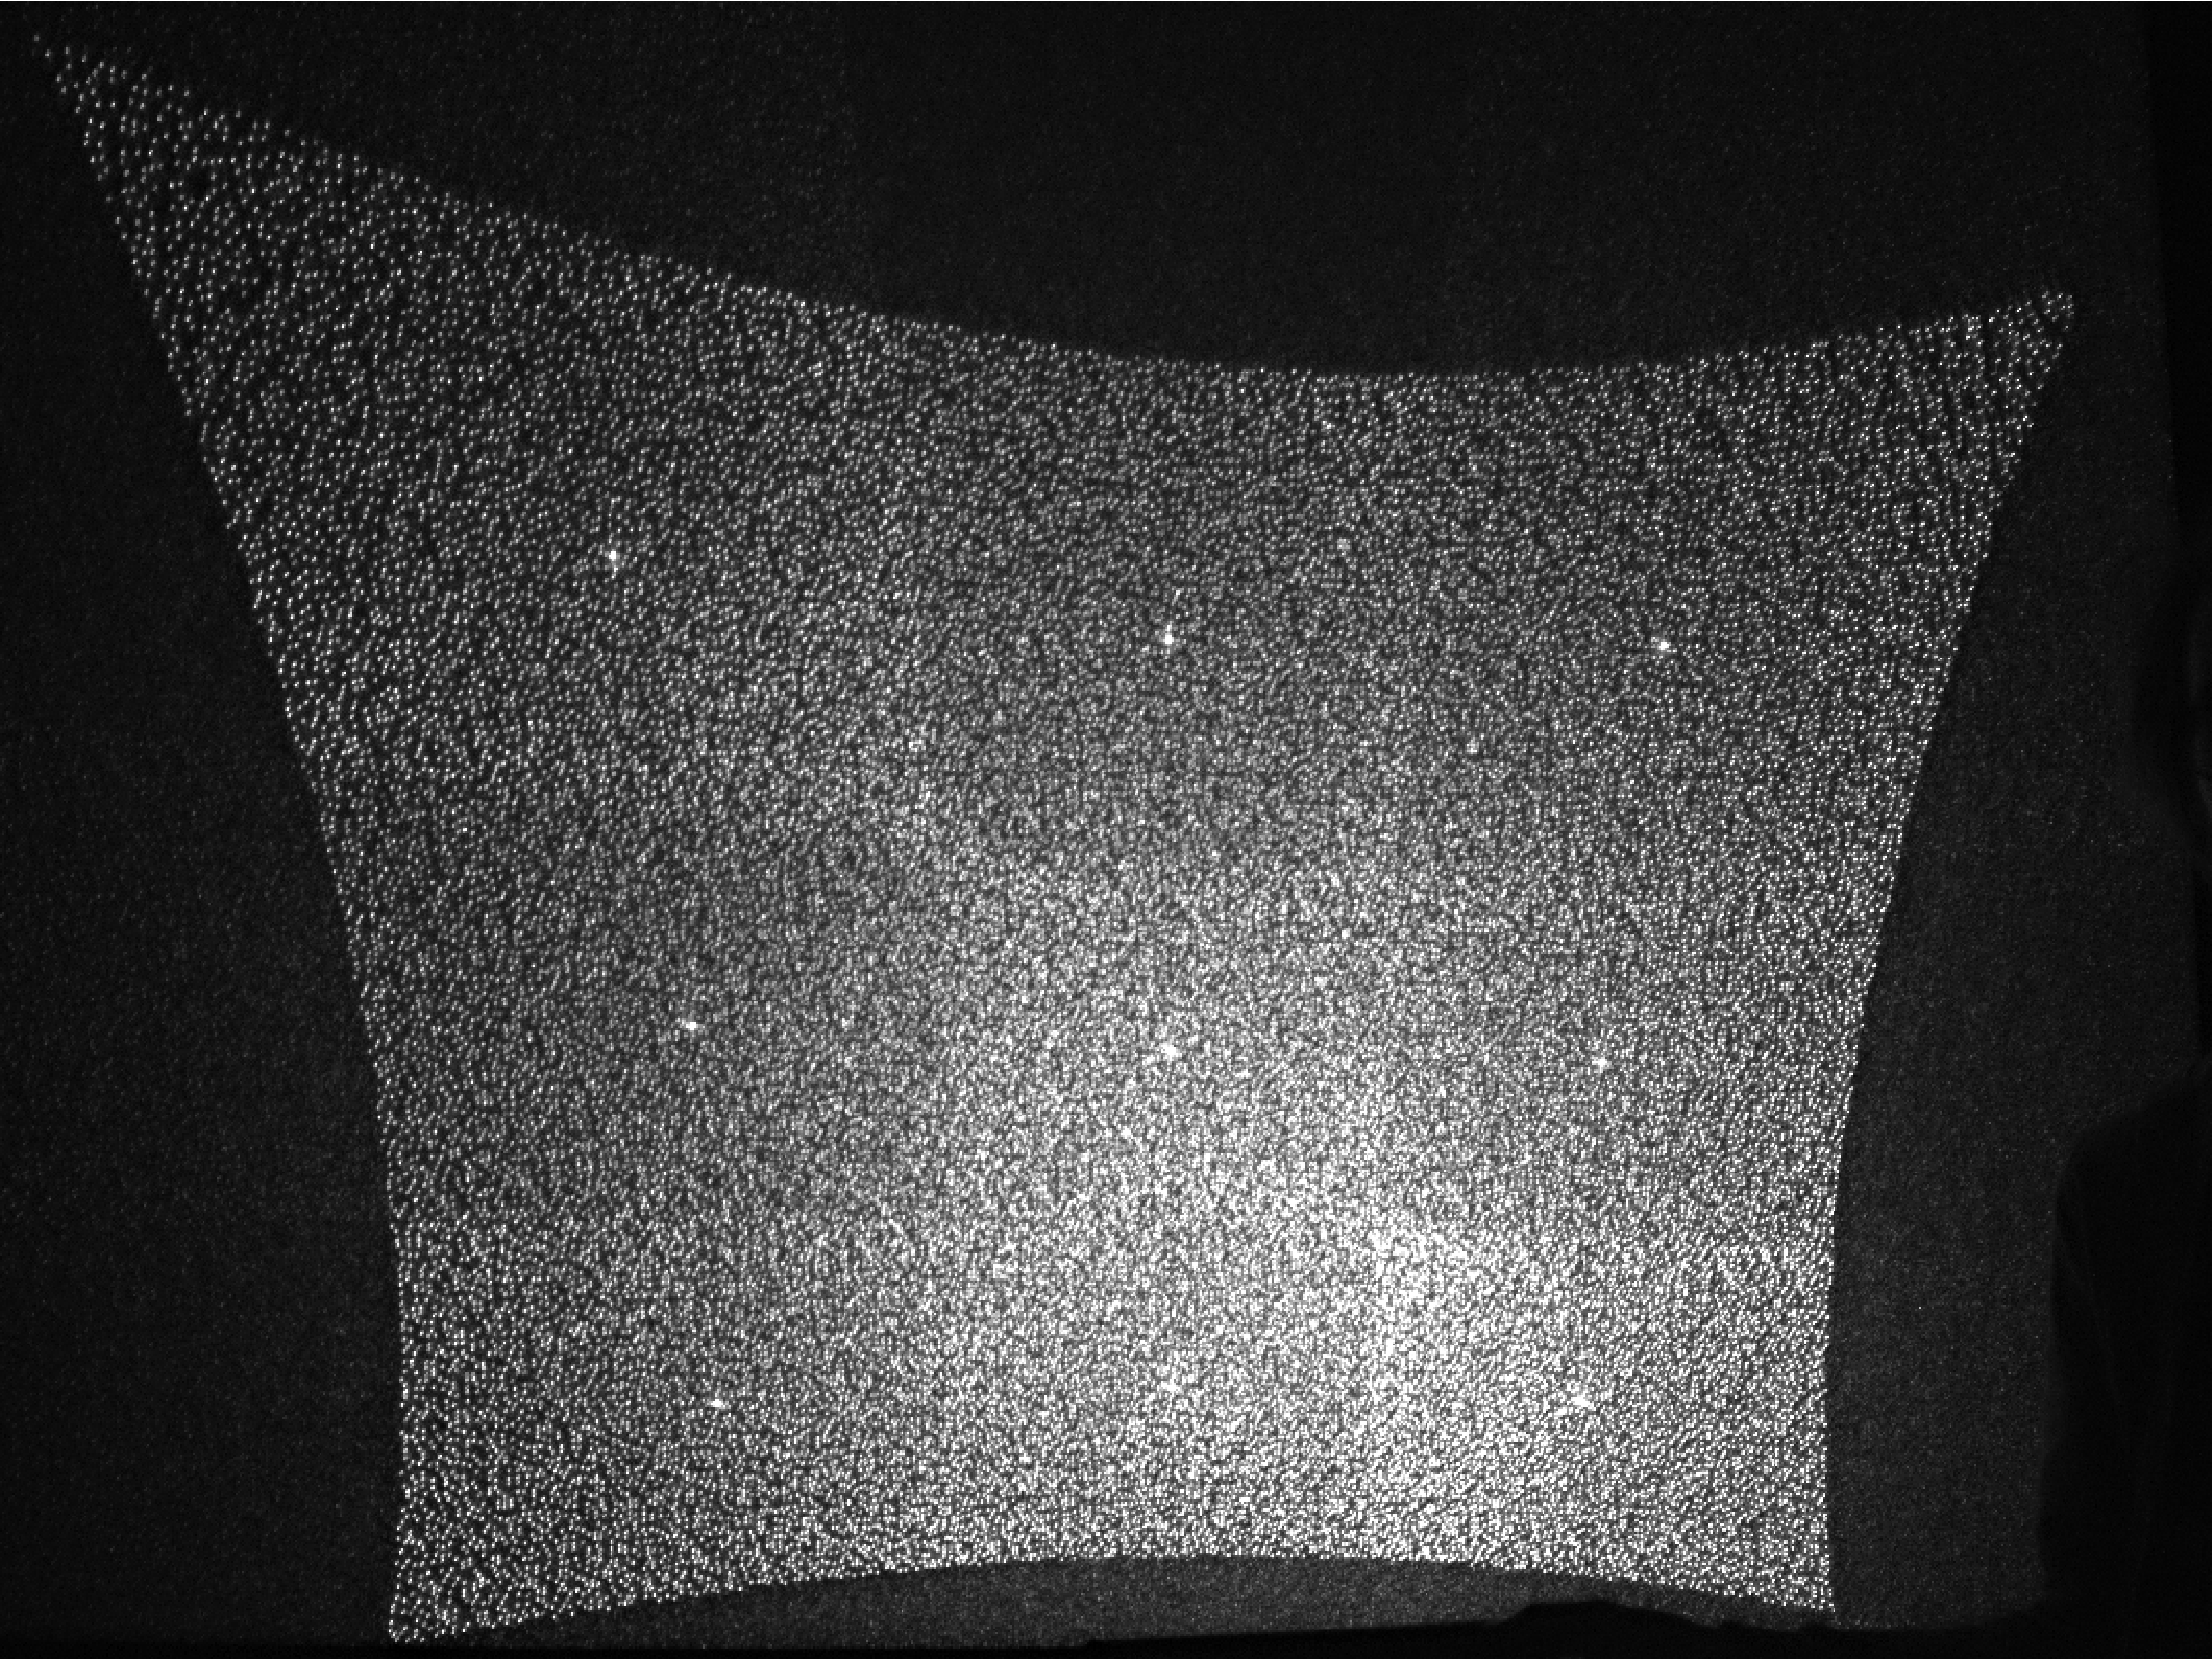
\includegraphics[width=1.0\textwidth]{images/whole_pattern.pdf}
        \caption{Near-infrared image of speckle pattern}
        \label{fig:pattern1}
    \end{center}
\end{figure}


\subsection{Stereo triangulation}
\label{sub:triang}

Evidence suggests that the kinect derives depth values using a proprietary
extension of the standard computer vision process known as stereo triangulation.
Figure~\ref{fig:triang} on page~\pageref{fig:triang} illustrates the general
principle, with an idealised configuration of two cameras, $c_{l}$ and $c_{r}$,
set up as a stereo unit, and a point, $p$, on an object viewed by both cameras.
In this model, we simplify: \begin{itemize}

    \item   the sensors as pinhole cameras;

    \item   the stereo set-up so that the cameras' normal lines are parallel;

    \item   the camera planes so these are ``flipped'' to the front of the focal points
    for ease of illustration.

\end{itemize}

\begin{figure}[ht]
    \begin{center}
        \begin{tikzpicture}[scale=0.75,cap=round]

    \def\xcl{-12}
    \def\xcr{-3}
    \def\yimageplanes{1}
    \def\imageplaneshalfwidth{1.5}

    % Styles
    \tikzstyle{axes}=[]

    \begin{scope}[style=axes]
    \draw[->] (0,0) -- (-15,0) node[below] {$x$};
    \draw[->] (0,0) -- (0,10) node[above] {$z$};
    \draw[->] (0,0) -- (0.5,-0.625) node[below] {$y$};

    \end{scope}

    % point on object
    \draw [fill] (-6.5,9) circle [radius=0.025];
    \draw node [above right] at (-6.5,9) {$p$};

    % left camera
    \draw [fill] (-12,0) circle [radius=0.025];
    \draw node [below left] at (\xcl,0) {$c_{l}$};
    \draw[-] (\xcl - \imageplaneshalfwidth,\yimageplanes) -- (\xcl + \imageplaneshalfwidth, \yimageplanes);

    % right camera
    \draw [fill] (-3,0) circle [radius=0.025];
    \draw node [below right] at (\xcr,0) {$c_{r}$};
    \draw[-] (\xcr - \imageplaneshalfwidth,\yimageplanes) -- (\xcr + \imageplaneshalfwidth, \yimageplanes);

    % depth plane
    %
    % image rays
    %
    % focal length
    %
    % depth
    %
    % camera distance
    %
    % left image normal offset
    %
    % right image normal offset
    %
    % inter-offset distance

\end{tikzpicture}

        \caption{``Standard'' stereo triangulation}
        \label{fig:triang}
    \end{center}
\end{figure}

The desired value is $Z_{p}$, i.e.\ the minimum distance from the $x-y$ plane to
$p$, or the ``depth measurement'' for that point. We obtain $Z_{p}$ from: 

\begin{itemize}

    \item the focal length ($f$);

    \item the inter-camera distance ($b$); and 

    \item the respective distances between left and right camera norms and the
    pixels corresponding to $p$ on the left and right image planes ($x_{l}$ and
    $x_{r}$),

\end{itemize}
using the similarity of triangles, which yields
%todo show algebra to derive this
\[
    \frac{Z_p}{b} = \frac{Z_p - f}{b - x_l + x_r}.
\]
Hence,
\[
Z_p = \frac {bf}{x_r - x_l}.
\]
The value $x_r - x_l$ is called the ``disparity''.

\subsection{Stereo triangulation: the Kinect way}
\label{sub:atriang}

Figure~\ref{fig:atriang} on page~\pageref{fig:atriang} shows the triangulation
model adapted, \emph{mutatis mutandis}, to a depth camera ($c$) projector ($s$)
pair. This is sometimes referred to as ``active triangulation''
\cite{alexander1987}, since one replaces one passive component (a camera) with
an active one (a projector). The same simplifications apply as in section
\ref{sub:triang}. The projector replaces the second camera here, and we
distinguish the target point ($p_a$) on the object plane from the corresponding
point ($p_r$) on a predetermined reference plane.

\begin{figure}[ht]
    \begin{center}
        \begin{tikzpicture}[scale=0.75,cap=round]

    % let's define some key values
    \def\xc{-12}
    \def\xs{-3}
    \def\yimageplanes{1.25}
    \def\imageplaneshalfwidth{1.5}
    \def\xdistoffsetf{\imageplaneshalfwidth  + 0.5}
    \def\xdistoffsetZa{\imageplaneshalfwidth  - 0.25}
    \def\xdistoffsetZr{\imageplaneshalfwidth  - 1.25}
    \def\ydistoffsetxl{\yimageplanes + 0.125}
    \def\ydistoffsetxr{\ydistoffsetxl}
    \def\ydistoffsetb{0}
    \def\ydistoffsetinterx{\ydistoffsetb}
    \def\xobject{-6.5}
    \def\objectdepth{5.5}
    \def\referencedepth{3 + \objectdepth}
    \coordinate (pa) at (\xobject,\objectdepth);
    \coordinate (s) at (\xs,0);
    \coordinate (c) at (\xc,0);
    \coordinate (rayl2) at (\xc,0);
    \coordinate (ipll) at (\xc - \imageplaneshalfwidth, \yimageplanes);
    \coordinate (iplr) at (\xc + \imageplaneshalfwidth, \yimageplanes);


    % intersections of normals and reference plane
    \coordinate (rnrdi) at (\xs, \referencedepth);
    \coordinate (lnrdi) at (\xc, \referencedepth);
    % intersections of normals and object plane
    \coordinate (rnodi) at (\xs, \objectdepth);
    \coordinate (lnodi) at (\xc, \objectdepth);

    \coordinate (pr) at (intersection of s--pa and lnrdi--rnrdi);

    % intersection of c -- pr and object plane
    \coordinate (cprodi) at (intersection of c--pr and rnodi--lnodi);

    % pixel on image plane and expected pixel on image plane
    \coordinate (pixel) at (intersection of ipll--iplr and pa--c);
    \coordinate (epixel) at (intersection of ipll--iplr and pr--c);

    % Styles
    \tikzstyle{axes}=[]

    \begin{scope}[style=axes]
    \draw[->, thick] (0,0) -- (-15,0) node (xaxis) [below] {$x$};
    \draw[->, thick] (0,0) -- (0,10) node (zaxis) [above] {$z$};
    \draw[->, very thick] (0,0) -- (0.5,-0.625) node [below] {$y$};

    \end{scope}

    % point on object
    \draw [fill, red] (pa) circle (0.05) node [above right] {$p_a$};

    % point on reference plane
    \draw [fill, purple] (pr) circle (0.05) node [above right] {$p_r$};

    % left camera
    \draw [fill, blue] (-12,0) circle (0.05) node [below left] {$c$};
    % left image plane
    \draw[-, thick] (\xc - \imageplaneshalfwidth,\yimageplanes) -- 
        (\xc + \imageplaneshalfwidth, \yimageplanes);

    % right camera
    \draw [fill, blue] (-3,0) circle (0.05) node [below right] {$s$};

    % depth plane
    \draw[dashed, domain=-16:2] plot (\x, {\objectdepth});
     
    % Reference plane
    \draw[dashed, domain=-16:2] plot (\x, {\referencedepth});
    % p_r

    % image ray
    \draw[dotted] (pa)--(c);

    % projection ray
    \draw[dotted] (pr)--(s);
    
    % expected image ray
    \draw[dotted] (c)--(pr);

    % image points
    \draw[fill, orange] (pixel) circle (0.05) node [below right] {$x$};

    % focal length
    \draw[<->, thick, gray] (\xc - \xdistoffsetf,0) -- (\xc - \xdistoffsetf,\yimageplanes)
        node [midway, left, gray] {$f$};
    
    % Camera norms
    % left
    \draw[->] (c) -- (\xc, \referencedepth + 1);
    % perpendicular symbol
    \draw[thick] (\xc,0.15) -| (\xc-0.15, 0); 
    % right
    \draw[->] (s) -- (\xs, \referencedepth + 1);
    % perpendicular symbol
    \draw[thick] (\xs,0.15) -| (\xs +0.15, 0); 
    %(\xs,0)
    
    % actual depth
    \draw[<->, thick, gray] (\xc - \xdistoffsetZa, 0)
        -- (\xc - \xdistoffsetZa, \objectdepth)
        node [midway, left, gray] {$Z_{a}$};
    % reference depth
    \draw[<->, thick, gray] (\xc - \xdistoffsetZr, 0)
        -- (\xc - \xdistoffsetZr, \referencedepth)
        node [midway, left, gray] {$Z_{r}$};
    
    % camera distance
    \draw[<->, very thick, gray] (\xc,\ydistoffsetb) -- (\xs,\ydistoffsetb)
        node [midway, below, gray] {$b$};
    
    % point disparity over epipolar line
    \draw[<->, very thick, gray] (cprodi) -- (pa) node [midway, above, gray] {$d_o$};
    % point disparity over image plane
    \draw[<->, very thick, gray] (epixel) -- (pixel) node [midway, above, gray] {$d_i$};
    
\end{tikzpicture}

        \caption{``Active'' stereo triangulation}
        \label{fig:atriang}
    \end{center}
\end{figure}

%todo uhm, notation for lines, again?
Now it is worth emphasising the order in which the Kinect proceeds: First, for
every image pixel $x_a$ corresponding to a point ($p_a$) registered by the depth
camera, the Kinect finds the matching reference image pixel $x_r$ corresponding
to a point ($p_r$) on the reference plane by solving the so-called
``correspondence problem'' discussed in section \ref{sub:corr}. Once a matching
reference point $p_r$ is found, the Kinect determines the disparity $d_i$ along
the $x$-axis in image space between the actual image of $p_a$ and the reference
image of $p_r$. With that obtained, is it possible to derive the desired ``depth
measurement'' $Z_a$ for the given point, or the minimum distance from the depth
camera's focal point to the object plane, from: 

\begin{itemize}

    \item the focal length ($f$);

    \item the inter-camera distance ($b$);

    \item the disparity between $x_a$ and $x_r$ along the x-axis ($d_i$);

    \item the reference image depth ($Z_r$),

\end{itemize}
using the similarity of triangles, which yields equations \ref{eq:atriang1} and
\ref{eq:atriang2}. Substituting for the common variable $d_o$, we simplify to
obtain equation \ref{eq:atriang3}.

%todo show algebra to derive this
\begin{align} 
    \frac{d_o}{b} = \frac{Z_r - Z_a}{Z_r} \label{eq:atriang1}\\
    \frac{d_i}{f} = \frac{d_o}{Z_a} \label{eq:atriang2}
\end{align}
\begin{equation} \label{eq:atriang3}
    Z_a = \frac{Z_r}{d_i \frac{Z_r}{b f} + 1}
\end{equation}

%todo: describe the issue of non-parallel cameras, epipolar lines, and how this
%is solved with image transformations.


\subsection{Correspondence problem}
\label{sub:corr}

In this section we highlight four potential solutions to the correspondence
problem, i.e.\ that of having to match subregions of the infrared camera images
with the corresponding subregions in one or more reference images stored in
memory. The coordinates of these pairs of subregions are necessary to derive
the disparity values, $d_i$, needed for the triangulation process described
above.  It is not unlikely that the Kinect implements some combination of these
and/or other methods, in order to solve the correspondence problem.

Note that, as implied in the triangulation approach described, matching occurs
along the horizontal axis only. So, the device successively attempts to match
subregions (of a fixed size) in the infrared image, by searching for the most
similar subregion along a horizontal band on either side of the subregion in
question. The axes in the image along which disparities occur as a function of
object depth are called the ``epipolar lines''. With parallel camera and
projector norms, these lines are parallel to the image $x$-axis. In case the
camera and projector are not lines up in this way, calibration and subsequent
image transformations can compensate.


\subsubsection{Scale-invariant transformations}

In order to recognise matching subregions across the actual and reference
speckle pattern images, the Kinect must overcome the fact that the scale of the
patterns varies with depth. One approach to dealing with this, is to match
scale-invariant representations of the respective sets of subregions. A class of
transformation functions, the Mellin transform(ref), is widely used in computer
vision to create such scale-invariant representations of an image. Much as the
Fourier transform of a function does not vary as one shifts that function along
its domain, the Mellin transform of a function equals the Mellin transform of a
scaled version of that function (c.f.\ (strongly simplified)
equation~\ref{eq:mellin1}).

\begin{equation} \label{eq:mellin1}
    M (f) = M(scale(f))
\end{equation}

The scale invariance of the Mellin tranform of an image holds only for scaled
images sharing the same centre point. A device using this approach to the
correspondence problem would need to store the Mellin transforms of all
subregions, of a given size, of a reference image of the speckle pattern. The
device would then use a correlation algorithm to compare these stored values
with the Mellin transforms of subregions to either side of the target point
along the epipolar line. The highest match would yield the coordinates of $x_r$.


\subsubsection{Coded light}

The coded light technique helps solve the correspondence problem in active
stereo triangulation set-ups. It is in fact a large class of techniques in which
information is encoded in some combination of colour and/or luminance and/or
patterns of shapes in the projected image. The information enables the
reconstruction of a subregion's coordinates in the projected image, when viewing
the projection of the image in a scene.

Since neither our own experiments, nor any of the patents and articles that we
reviewed suggested any significant colour or luminance differentiation in the
Kinect's use of its projected speckle pattern, we conclude that any use of light
coding would rely on patterns alone.

A simple example of a light coding technique involving patterns would encode de
Bruijn sequences in patterns of vertical stripes %, as shown in
%figure~\ref{fig:debruijn} (page~\pageref{fig:debruijn}, 
allowing for horizontal
localisation. A variety of light coding that evokes the Kinect's grid of
speckles (c.f.\ figure~\ref{fig:speckle}, page~\pageref{fig:speckle} that of
``pseudo-random binary arrays'' of light (c.f. figure~\ref{fig:prba},
page~\pageref{fig:prba}) \cite{geng2011structured}).

\begin{figure}[ht]
    \begin{center}
        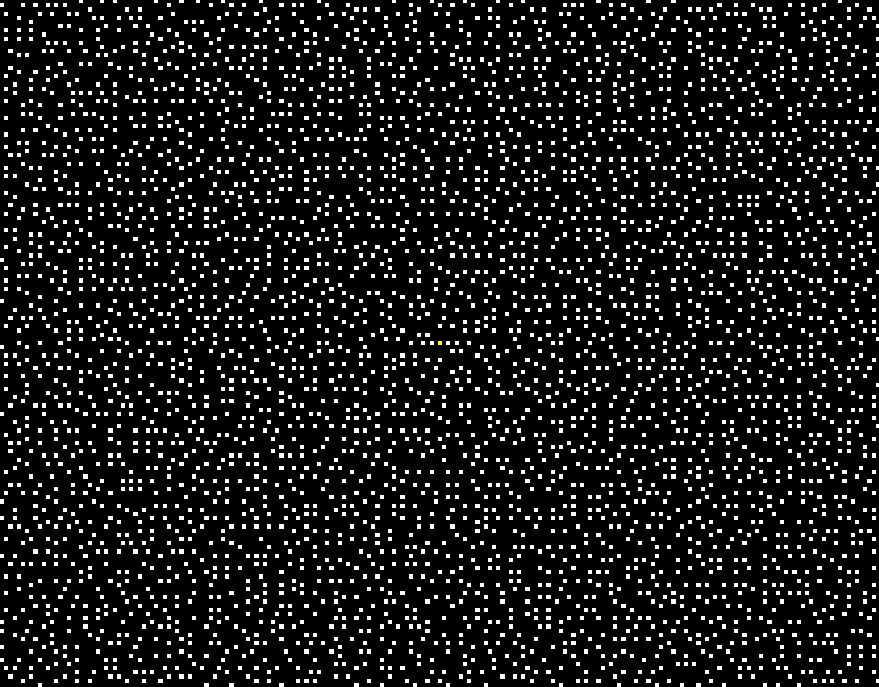
\includegraphics[width=1.0\textwidth]{images/speckle.pdf}
        \caption{Kinect speckle pattern}
        \label{fig:speckle}
    \end{center}
\end{figure}


\begin{figure}[ht]
    \begin{center}
        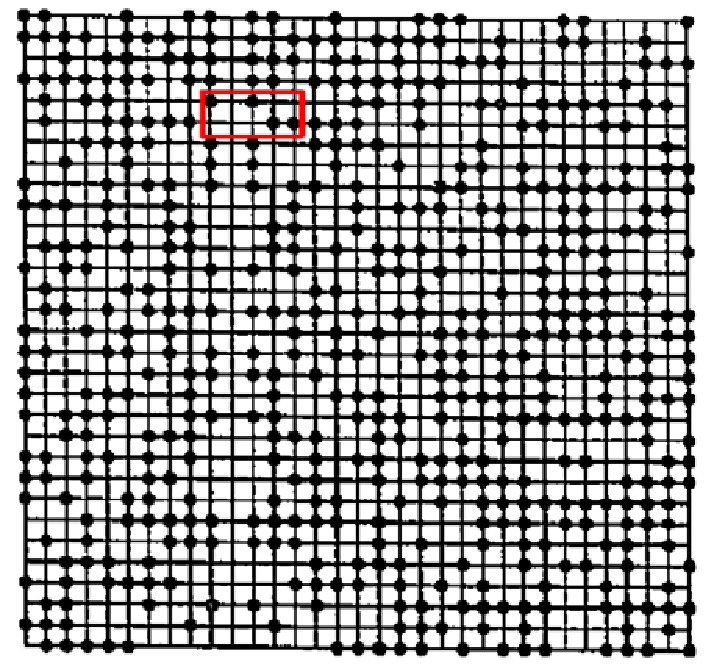
\includegraphics[width=1.0\textwidth]{images/prba.pdf}
        \caption{Light coding by Pseudo Random Binary Array}
        \label{fig:prba}
    \end{center}
\end{figure}


\subsubsection{Scale identification}

In this approach, the speckle pattern is constructed so that the average
distance from any given speckle so a set number of nearest speckles has a
predetermined relation to the scale of the image. Once this is established, the
image is altered to match the reference image's scale, whereafter correlation is
performed for each subregion along its horizontal band to obtain a corresponding
region in the reference image.


\subsubsection{Multiple reference images}

Finally, it is possible that the Kinect in fact holds a number of reference
images of the speckle pattern of different scales. Correlation based matching
could then be carried out in parallel, for example using a chip optimised for
such a parallel task, for find corresponding subregions. Note that the speckle
pattern would then need to be configured so that there are no significantly
similar subregions across the various scales of reference image.

%todo describe experiment with pictures... 

%\subsubsection{Experiment: pattern variation over distance}

%todo describe experiment with pictures... (first discuss whether useful with Jeroen)



%\section{Precision of the intrument}
%\label{precision}

%todo: just take data from article
%In this section we describe the Kinect's characteristics as a depth measurement
%tool, and notably the precision of the measurements.


%\subsection{Depth precision}
%
%\subsubsection{Sources of error}
%
%\subsection{Depth image resolution}
%
%\subsubsection{Sources of error}
